\section{Monitoring du bus mémoire}\label{sec:yamb}


Cette section présente le développement de notre outil \verb=YAMB= (\textit{Yet Another Memory Bandwidth profiling tool}). \verb=YAMB= mesure l'activité des différents contrôleurs mémoire (en lecture et en écriture) ainsi que le nombre d'évènements \textit{\gls{miss}} dans le dernier niveau de cache (LLC). L'évolution du trafic mémoire peut ensuite être affiché sous forme de graphique (voir \autoref{pic:yamb_stream}). L'outil propose l'utilisation d'une librairie, permettant d'annoter facilement certaines zones du code pour faciliter la lecture du graphique.

\begin{figure}[h!]
\center
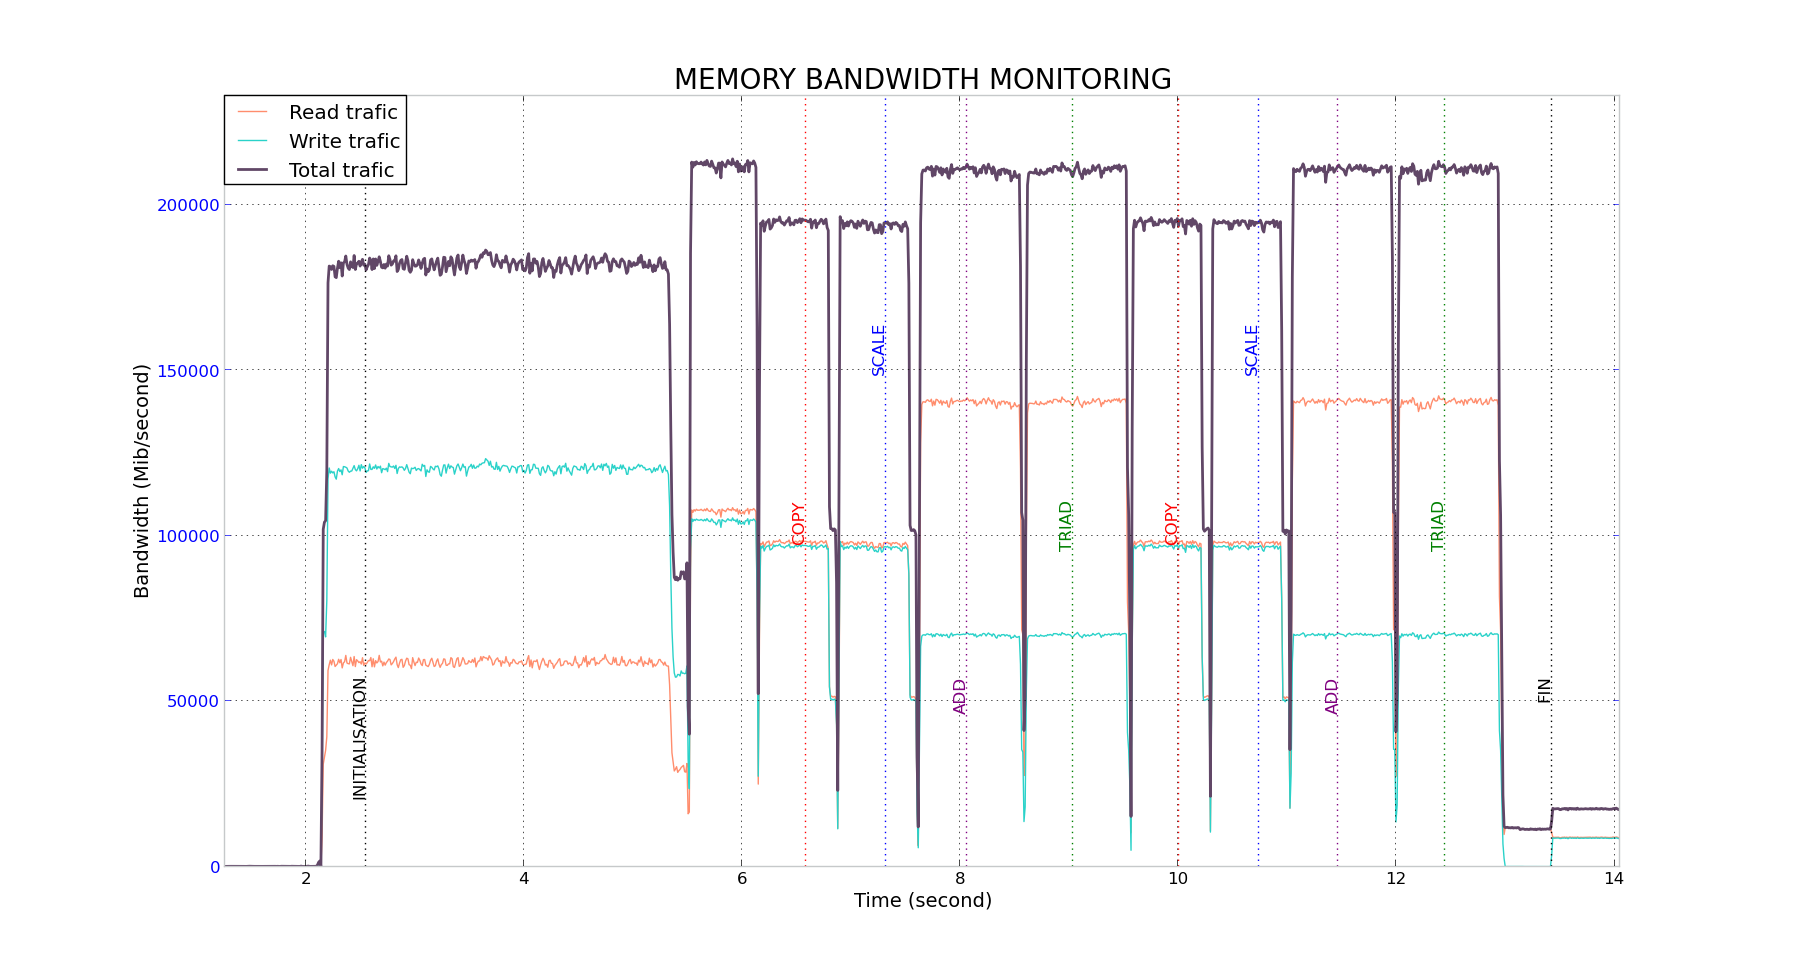
\includegraphics[width=16cm]{images/yamb_stream.png}
\caption{\label{pic:yamb_stream} Exemple d'utilisation de l'outil \texttt{YAMB} pour suivre l'activité du bus mémoire lors de l'exécution du benchmark \texttt{STREAM} \cite{McCalpin1995} pour deux itérations des 4 noyaux de calculs: \texttt{copy}, \texttt{scale}, \texttt{add} et \texttt{triadd}.}
\end{figure}
\textbf{TODO rogner + 16 CM}




\subsection{Introduction}
%%%%%%%%%%%%%%%%%%%%%%%%%%%%%%%%%%

    \subsubsection{Motivation et objectifs}
     %%%%%%%%%%%
     
        La majorité des processeurs utilisés en HPC utilisent une architecture Von Neuman (voir \aref{sec:vonneumann}). Pour la majorité des applications de calculs intensifs \cite{Drepper2007}, le système mémoire de ces architectures est le principale responsable de la limitation des performances. Nous observons une augmentation du nombre de coeurs sur les processeurs de dernière génération sans réelle évolution de la performance de cette ressource critique. Cette disparité résulte en une augmentation d'accès concurrents au bus mémoire, limitant la performance des applications. De plus, ce bus étant une ressource partagée par les coeurs d'un même processeur, la mauvaise utilisation de celui-ci par un coeur affecte la performance des autres.
        
        La majorité des applications HPC étant limitée par la performance du bus mémoire, il est primordial de valider l'utilisation optimale du bus mémoire. Pour cela, il est nécessaire de vérifier qu'il est utilisé à son débit maximal (saturation) mais aussi de l'efficacité des transferts réalisés (transferts de données utilisées par le processeur). 
        Pour réaliser ces vérifications, il n'est pas envisageable de mesure le débit mémoire moyen lors de l'exécution de l'application ou même d'un \gls{kernel}. En effet, une application peut être limitée par la performance du bus, sans que celui-ci soit saturé sur la totalité de l'exécution du code. Par exemple, si les accès sont tous réalisés au même moment, le bus peut être saturé pendant un court instant et être ensuite inutilisé. Sur la totalité de l'exécution, on obtiendra une mesure qui indiquera que le bus n'est pas saturé alors qu'il s'agit bien du goulot d'étranglement des performances de l'application.
        
        %Le bus mémoire étant une ressource critique, il doit être utilisé pour transférer le plus possible de données utiles. Les transferts entre la mémoire et le processeur se font  par paquet (ligne de cache). Il est primordial que le maximum des données présent dans cette ligne de cache soit utilisées pour un calcul lorsque celle-ci est transférée vers le processeur. Pour cela, une adaptation des structures de données peut être nécessaire.
    
        L'objectif de l'outil présenté dans cette section est de répondre aux deux prérogatives indiquées ci-dessus: saturation du bus et utilisation effective. Pour y répondre, l'utilisateur doit posséder un outil lui permettant de suivre son activité avec une résolution fine (de l'ordre de la milliseconde). L'outil en question doit pouvoir distinguer les accès réalisés en lecture et en écriture pour pouvoir s'assurer de l'utilisation effective du bus. Nous expliquons comment la rapport entre les quantités de données en lecture et en écriture peut être utilisé pour mesurer la performance d'un code dans la \autoref{sec:smm}.

    \subsubsection{Verrous et état de l'art}
    %%%%%%%%%%%
        
        La principale difficulté pour le développement d'un tel outil vient de l'utilisation des compteurs matériels permettant de compter les évènements relatifs aux accès mémoires. Ces compteurs permettent de compter les évènements se produisant sur un processeur et sont présentés dans l'\aref{annexe:hardware_counter}. Ils sont accessibles par le biais de composants appelés \gls{PMU}. Un processeur moderne possède généralement au moins deux familles de PMU : une PMU \textit{oncore} situé sur chaque coeur du processeur et une PMU \textit{uncore} située directement sur le processeur. Comme étudié dans la \aref{sec:edl_perf_uncore}, les compteurs  responsables du comptage des évènements liés aux transferts mémoires sont situés sur les PMU \textit{uncore}. Sur des architectures modernes telles que les processeurs Intel Skylake, ces compteurs comptent les accès mémoire réalisés en distinguant la lecture de l'écriture.
        
        Mis à part certaines tâches, comme la gestion des pages, les accès mémoire sont réalisés directement par le contrôleur mémoire. Le système d'exploitation n'a généralement pas connaissance de l'évolution de ces accès, contrairement à d'autres ressources comme les \textit{entrées/sorties} (I/O) pour lesquelles le système d'exploitation joue le rôle d'intermédiaire avec l'application. Ainsi, comme les compteurs ne sont associés à aucun coeur, il est impossible de faire correspondre un accès mémoire au coeur et donc au processus qui en est responsable. Pour des outils nécessitant une grande précision \cite{Larysch2016a}, l'utilisation de ces compteurs n'est donc pas possible. Notre outil a pour objectif d'analyser l'activité d'applications HPC qui utilisent généralement tous les coeurs des processeurs pour la même application. Cette particularité n'est donc pas un verrou majeur pour notre développement.  
 
        La programmation des PMU varie d'une architecture à l'autre, ce qui les rend difficiles à programmer et à maintenir. Que ce soit pour le \textit{core} ou le \textit{uncore}, ces méthodes sont assez complexes à utiliser et à maintenir. C'est pourquoi il est courant d'utiliser des interfaces de haut niveau telles que \texttt{PAPI} \cite{Browne2000} ou \texttt{perf} qui permettent de ne plus dépendre de l'implémentation des compteurs à bas niveau. 
        Ces interfaces ont permis le développement de nombreux outils (voir \autoref{sec:edl_monitoring_tools}). Intel propose \verb|VTune| \cite{reinders2005vtune} et Intel \verb=MBM= \footnote{Intel MBM - \url{https://github.com/intel/intel-cmt-cat/wiki}}. Le premier est un outil propriétaire nécessitant une licence payante. Le deuxième est proposé en libre accès sur le dépôt en ligne d'Intel mais n'est compatible qu'avec des architectures Intel.
        D'autres outils tels que \verb=TAU= \cite{Lindlan2000} ou \verb=Extrae= \cite{Rodriguez} présentent de nombreuses informations à l'utilisateur qui rendent difficile la compréhension des résultats. De plus, ce grand nombre d'informations nécessite généralement l'utilisation de plusieurs compteurs matériels qui peuvent ne plus être présents d'une architecture à l'autre. La complexité des outils peut aussi les rendre dépendants de librairies externes non compatibles avec certaines architectures rendant leur utilisation impossible (\verb|MAQAO| \cite{Djoudi2005}). 
        D'autres travaux tels que \verb=Memguard= \cite{Yun2013} mesurent le nombre de \textit{\gls{miss}} dans le dernier niveau de cache pour en déduire le trafic du bus mémoire. Malheureusement, avec la complexification des architectures et l'utilisation constante des unités de préchargement mémoire, certains transferts mémoires sont réalisés avant qu'un évènement \textit{\gls{miss}} ne soit déclenché. Il n'est donc plus possible de mesurer le trafic mémoire avec ces techniques-là. 
        
        %L'outil \textit{Likwid} \cite{Treibig2010} propose de mesurer les données transférées (GB) et leur débit (GB/s) pour un noyau de calcul. Il peut aussi générer des traces pour suivre plus précisément l'utilisation du bus mémoire. mais l'outil de visualisation des données n'est plus supporté.
        
        %Les moyens disponibles pour les programmer sont complexes et propres à chaque architecture. Le développement d'un outil utilisant une programmation directe des compteurs rend très difficile la portabilité de l'outil sur différentes architectures.
   

\subsection{Développement de YAMB}
%%%%%%%%%%%%%%%%%%%%%%%%%%%%%%%%%%

       De nombreux outils et interfaces ont été développés pour accéder aux compteurs matériels avec leurs avantages et leurs inconvénients. Les principales contraintes des outils développés au cour de ce travail de thèse sont la portabilité et l'accès libre aux sources. Après avoir testé les différents outils et interfaces disponibles, nous avons choisis de baser le développement de \verb|YAMB| sur \texttt{Perf Events} \cite{Weaver2013} (voir \autoref{sec:edl_profiling_perf}).
       
    \subsubsection{Perf Events}
        
            Contrairement à d'autres outils tels que \texttt{Likwid} \cite{Treibig2010} ou \verb=PAPI= \cite{Browne2000}, le système de suivi de performance \texttt{Perf Events} fait parti du projet Linux. Son intégration dans le noyau nous assure un maximum de disponibilité dans les environnements de calcul haute performance ainsi qu'un maximum de compatibilité avec les architectures émergentes.  La principale difficulté de \texttt{Perf Events} vient l'utilisation de l'appel système \textit{perf\_event\_open} qui permet de programmer les compteurs matériels \cite{Selva2017}. S'il permet d'éviter à l'utilisateur d'écrire manuellement les différents bits de configuration des registres, beaucoup de travail reste à faire pour le développeur désireux de profiler ses applications. En effet, Linux supporte de nombreux processeurs possédant différentes versions de PMU, les développeurs du noyau ont donc laissé la programmation bas niveau à l'utilisateur. En conséquence, cet appel système est très complexe à utiliser et ne peut pas être utilisé de manière portable. Les principales difficultés consistent à trouver les événements à compter ou à échantillonner, à configurer tous les paramètres à transmettre à l'appel système et à effectuer plusieurs appels système en fonction du nombre de \textit{threads} de l'application profilée et du nombre de coeurs utilisés. Ces différentes difficultés (programmation, portabilité) ont été les principales motivations du développement d'autres outils tels que \verb=PAPI= \cite{Browne2000}, \verb=Intel PCM=\footnote{Intel Performance Counter Monitor - \url{https://software.intel.com/en-us/articles/intel-performance-counter-monitor}} ou \verb=NUMAP= \cite{Selva2017}.

            En plus de l'appel système, \texttt{Perf Events} fournit un outil accessible depuis l'espace utilisateurs lui permettant de contrôler le profilage. Nommé \texttt{perf}, ce programme utilise l'interface noyau pour réaliser des mesures soit en échantillonnage soit en comptage (voir \autoref{sec:hc_counting_sampling}). Comme présenté dans la \autoref{sec:edl_profiling_perf}, \textit{perf} est l'outil de profilage de Linux, et nous espérons que sa large disponibilité rendra notre outil facilement utilisable par le plus grand nombre de personnes. Bien qu'il s'agisse avant tout d'un outil d'espace utilisateur, la commande \verb=perf= fait partie du noyau Linux du point de vue du développement. Faire partie de Linux assure une haute exigence du développement du code ainsi qu'un support au fil des versions du noyau. En raison des permissions limitées possédées par les utilisateurs de supercalculateur, l'outil doit utiliser une interface ne nécessitant pas de droits privilégiés (\textit{root}) pour fonctionner. Du fait du développement de l'interface \verb=perf_event= dans le code noyau, il est possible pour l'administrateur d'autoriser les utilisateurs normaux à accéder aux compteurs. Cela peut être fait en écrivant la valeur 1 dans le fichier \verb=/proc/sys/kernel/perf_event_paranoid=.
            Lorsque le noyau supporte le nom symbolique des évènements, \texttt{perf} est très simple à utiliser. Dans le cas contraire, \texttt{Perf Events} offre la possibilité aux utilisateurs expérimentés d'encoder leurs propres évènements.
                
            
    \subsubsection{Fonctionnement de l'outil YAMB}
    %%%%%%%%%%%%%%%%%%%%%%%%
     
         La commande \verb=perf= peut être utilisée pour programmer les \gls{PMU} \textit{uncore} et accéder aux compteurs des contrôleurs mémoires. L'outil \verb=YAMB= utilise cette commande pour configurer les PMU pour qu'elles comptent les transactions en cours sur chaque canal mémoire, en lecture et en écriture. La commande peut aussi être utilisée pour compter le nombre d'évènements \textit{\gls{miss}} dans le cache de dernier niveau.
        
        Le lancement de la commande \verb=perf= en arrière-plan et le traitement des données dans un fichier de sortie constituent le coeur de l'outil de profilage \verb=YAMB=. Ensuite, un script peut être utilisé pour dessiner le graphique. 
        L'outil \verb=YAMB= reçoit deux options \verb=--start= et \verb=--stop=. L'utilisation de la première option lance la commande \verb|perf| avec les arguments adéquats en arrière-plan. L'appel du script avec l'option \verb=--stop= s'occupe de retrouver le \verb|PID| du processus de \verb|perf| pour l'arrêter et de sauver les données collectées dans un fichier. Entre ces deux appels, l'utilisateur peut exécuter son application ou attendre un certain temps:
\begin{lstlisting}[language=bash]
$ ./yamb.sh --start
$ ... sleep | run application ...
$ ./yamb.sh --stop
\end{lstlisting}
        Comme le montre l'extrait de code ci-dessus, l'avantage de cet outil réside dans la flexibilité de son utilisation. Il est courant dans le travail d'analyste de vouloir suivre l'exécution d'une application pendant une période donnée. L'exécution de celle-ci pouvant durer plusieurs heures, il est important que notre outil ne nécessite pas d'attendre son exécution complète pour prodiguer ses résultats. Grâce à cette approche, l'utilisateur se connecte à un serveur durant l'exécution de l'application, lance l'outil pendant une période voulue et l'arrête pour analyser les résultats. Cette méthodologie permet de laisser l'application s'exécuter. Le code de l'application pouvant être instrumenté pour annoter le graphique de résultat, il est possible de tracer et d'identifier les parties du programme mesurées par l'outil.
        

    \subsubsection{Annotation}
    %%%%%%%%%%%%%%%%%%%%%%%%

        Pour aider à identifier la zone de code responsable du trafic mémoire, une librairie a été développée. Elle permet d'annoter le code d'une application (\verb=c=, \verb=c++= et \verb=fortran=) à l'aide d'un \verb=label= et d'une \verb=couleur=. La librairie ne contient que la fonction \verb=yamb_annotate_set_event= permettant d'écrire ces informations dans un fichier de journal:
\begin{lstlisting}[label=lst:yamb_api ,language=C]
int yamb_annotate_set_event(const char * label, const char *couleur){
...
    m_LOG_FILE << time_step << " " << label << " " << couleur << endl;
...
}
\end{lstlisting}


    \subsubsection{Mesure de l'impact sur la performance}
    %%%%%%%%%%%%%%%%%%%%%%%%
        Un défaut majeur des outils de mesure de performance est leur impact sur la performance de l'application étudiée. Nous avons réalisé plusieurs tests avec différentes fréquences d'échantillonnage pour estimer l'impact de \verb|YAMB| sur l'application mesurée. Même lorsque la fréquence la plus rapide soutenable par \verb=perf= est utilisée (100Hz), l'impact sur la performance est très faible (inférieur à 5\%). Pour une étude suffisamment précise de l'application, obtenir 100 mesures par seconde semble largement suffisant. Nous considérons que cette baisse de performance est suffisamment faible pour s'assurer que la performance mesurée est proche de la performance réelle.
     
    
    
    
\subsection{Utilisation}
%%%%%%%%%%%%%%%%%%%%%%%%%%%%%%%%%%
 

        Cette section présente un exemple d'utilisation de \verb=YAMB= appliqué au benchmark \verb=STREAM= \cite{McCalpin1995}. Pour mieux comprendre l'évolution du trafic mémoire, la première étape est d'annoter les différentes parties du code intéressantes. Pour cela, nous utilisons la fonction \verb=yamb_annotate_set_event= pour ajouter une trace sur le graphique lors de chaque début de benchmark. L'analyse peut ensuite être lancée avec les commandes suivantes:
    
\begin{lstlisting}[label=lst:yamb_use ,language=C]
$ ./yamb.sh --output log_stream --command ./stream.SKL.192GB
$ python ./format_log.py --data log_stream.perf.mem --annotate log_stream.annotate
\end{lstlisting}

        Le résultat de cette première expérimentation peut être vu sur la \autoref{pic:yamb_stream}. L'utilisation du graphique peut ensuite permettre d'agrandir les parties plus intéressantes comme le noyau de calcul \verb=triad= (voir \autoref{pic:yamb_stream_triad}). Grâce à la distinction entre les accès mémoire réalisés en lecture ou en écriture, nous pouvons remarquer que le ratio de transfert obtenu de deux lectures pour une écriture est bien celui attendu pour le noyau de calcul étudié (voir \autoref{sec:methodo_step3}).
        
        
        \begin{figure}
        \center
        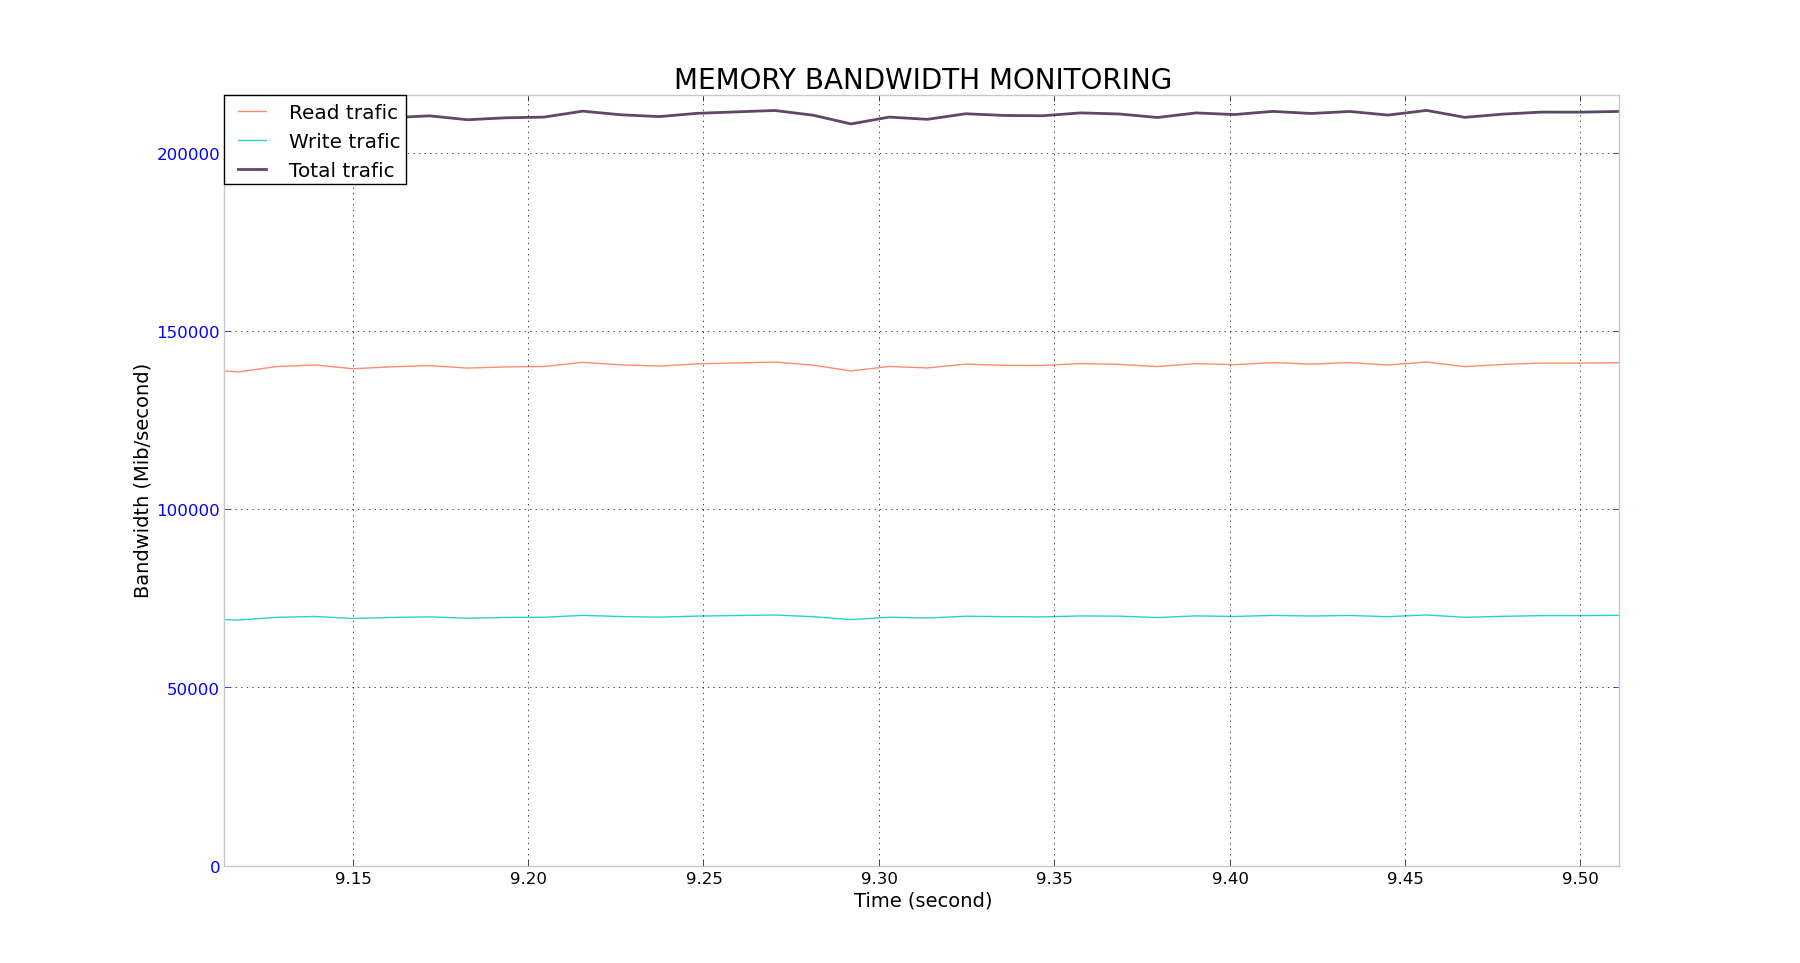
\includegraphics[width=14cm]{images/yamb_stream_triad.png}
        \caption{\label{pic:yamb_stream_triad} Trafic mémoire mesuré en Mb/s lors de l'exécution de la fonction \texttt{triad} du benchmark \texttt{STREAM}.}
        \end{figure} \textbf{todo plus grand}
        \textbf{todo check MB vs mb ???}

     
        \paragraph{Autres utilisations.} L'outil \verb|YAMB| est utilisé à plusieurs reprises dans ce manuscrit de thèse. Une utilisation est réalisée avec le benchmark \verb=dml_mem= pour caractériser la capacité du cache de dernier niveau à stocker un jeu de données dont la taille s'approche de celle du cache (\autoref{sec:dml_large_page}). Une autre utilisation est présentée dans le \autoref{chap:methodo} pour illustrer l'application de la méthodologie et l'utilisation des ratios de lecture et écriture pour s'assurer de l'optimalité d'un code.
        
     